% This goes at the from of the file - you can select different things here like 12pt, 11pt, paper size, double sided etc.

\documentclass[a4paper,11pt]{article}

% Packages for different settings - there are many of these you can access by googling (item you want and latex).
\usepackage{amsfonts}
\usepackage{pifont}
\usepackage{graphicx}
\usepackage{amsmath}
\usepackage{enumerate}
\usepackage{epsfig}
\usepackage{latexsym}
\usepackage{amssymb}
\usepackage{color}
\usepackage{amscd}
\usepackage{natbib}
\usepackage{multirow}
\usepackage{graphicx}
\usepackage{lscape}
\usepackage{float}
\usepackage{bm}

%%%%%%%%%%%%%%%%%%%%%%%%%%%%%%%%
% paper margins settings.
\pagestyle{plain}  
\oddsidemargin0cm
\hoffset-1cm
\voffset-0.5cm
\topmargin-1.4cm 
\textheight25cm \textwidth18cm \parindent0.5cm
%%%%%%%%%%%%%%%%%%%%%%%%%%%%%%%%


\begin{document}
\title{Assignment 1: MATH3911}
\author{Alexander Kwok$^{1}$  
\\$^{[1]}${\small email:
z3332883@zmail.unsw.edu.au; } 
}

\date{\textbf{Assignment 1:} Version from \today }

\maketitle
This assignment is my own work. I have read and understood the University Rules in respect to Student Academic Misconduct.
\section{Question 1}
\begin{enumerate}[(a)]
	\item
		$W = I_{\{X_1=2 \}}(\bf{X})$ is a simple unbiased estimator of $\tau (\lambda)$ since $E(W)= 1\times Pr(X_1=2) = \frac{\lambda^2e^{-\lambda}}{2!}$
	\item
		By rearranging the probability density function of Poisson Distribution:
		\[f(x;\lambda)=\frac{e^{-\lambda}\lambda^x}{x!} = \frac{e^{-\lambda}}{x!}e^{xlog\lambda} =a(\lambda)b(x)exp\{c(\lambda)d(x)\}
		\]
		It is clear that $a(\lambda) = e^{-\lambda}, b(x) = \frac{1}{x!}, c(\lambda) = log \lambda$ and $d(x) = x$. Therefore, the distribution belongs to 1-parameter-exponential family. So the statistic $T = \sum^n_{i=1} d(X_i) = \sum^n_{i=1} X_i$ is complete and minimal sufficient for $\lambda$.
		\\Then in order to derive the UMVUE of $\tau (\lambda)$, we use the Lehmann-Scheffe theorem which states that $E(W|T)$ is the unique UMVUE of  $\tau (\lambda)$
		\\Hence we can obtain the UMVUE by finding $E(W|T)$,
		\\Note that $X \sim Poi(\lambda) , T =  \sum^n_{i=1} X_i \sim Poi(n\lambda) ,  \sum^{n-1}_{i=2} X_i \sim Poi((n-1)\lambda)$
		\begin{align*}
			E(W|T=t) &= E(X_1=2 |  \sum^n_{i=1} X_i=t) \\
			&= \frac{P(X_1=2  \cap \sum^{n-1}_{i=1} X_i=t-2)}{P(T=t)}\\
			&= \frac{P(X_1=2 )P( \sum^{n-1}_{i=1} X_i=t-2)}{P(T=t)}\\
			&= \frac{ \frac{\lambda^2e^{-\lambda}}{2!} \times  \frac{[(n-1)\lambda]^{t-2}e^{-(n-1)\lambda}}{(t-2)!}}{ \frac{(n\lambda)^te^{n\lambda}}{t!}}\\
			&= \frac{t!(n-1)^{t-2}}{2(t-2)!n^t}\\
			&= \frac{t(t-1)(n-1)^{t-2}}{2n^t}\\
			&= \frac{t(t-1)}{2n^2} \bigg(1-\frac{1}{n}\bigg)^{t -2}
		\end{align*}
		Hence, by Lehmann-Scheffe theorem , $E(W|T=t)= \frac{t(t-1)}{2n^2} \bigg(1-\frac{1}{n}\bigg)^{t-2}$ is the UMVUE for $\tau (\lambda)$
	\item
		First obtain the MLE of $\lambda $:
		\begin{align*}
			0 &= V(\bf{X},\hat{\lambda})\\
			&= -n + \frac{\sum^n_{i=1} X_i}{\hat{\lambda}}\\
			\hat{\lambda} &= \bar{X}
		\end{align*}
		Then using the transformation invariance property of the MLE, we can obtain the MLE $\hat{\tau}$ of $\tau(\lambda)$ which is,
		\[
		\hat{\tau} _{\bf{MLE}}= \tau(\hat{\lambda}) = \frac{\bar{X}^2e^{-\bar{X}}}{2!}
		\]
		Now as MLE is asymptotically normal, unbiased and efficient, so by delta method, the asymptotic distribution is
		\[
		\sqrt{n}(\hat{\tau} - \tau(\lambda)) \xrightarrow{d} N\bigg( 0 , \bigg[ \frac{\partial \tau(\lambda)}{\partial \lambda} \bigg]^2 I_{X_1}^{-1}(\lambda)\bigg)
		\]
		where
		\[
		\frac{\partial \tau(\lambda)}{\partial \lambda} = \frac{\partial}{\partial \lambda} \bigg(  \frac{\lambda^2e^{-\lambda}}{2!} \bigg) = \frac{2\lambda e^{-\lambda} - \lambda^2e^{-\lambda}}{2} = \lambda (2-\lambda) \frac{e^{-\lambda} }{2}
		\]
		and
		\[
		I_{X}(\lambda) = E\bigg(-\frac{\partial}{\partial \lambda} V(\bf{X},\lambda) \bigg) = E\bigg(-\frac{\partial}{\partial \lambda} \bigg( -n + \frac{\sum^n_{i=1} X_i}{\hat{\lambda}} \bigg) \bigg) = E\bigg(  \frac{\sum^n_{i=1} X_i}{\hat{\lambda}^2} \bigg) = \frac{n}{\lambda}
		\]
		therefore
		\[
		I_{X_1}(\lambda) = \frac{1}{\lambda}
		\]
		Substitute all the calculation back we obtain the distribution as follow:
		\[
		\sqrt{n}(\hat{\tau} - \tau(\lambda)) \xrightarrow{d} N\bigg( 0 , \bigg[ \lambda (2-\lambda) \frac{e^{-\lambda} }{2}\bigg]^2 \lambda \bigg)= N\bigg(0, \frac{\lambda^2(2-\lambda)e^{-2\lambda} }{4}\lambda \bigg) = N\bigg(0, \frac{\lambda^3(2-\lambda)e^{-2\lambda} }{4} \bigg)
		\]
	\item
		From the data we can obtain $\bar{X} = \frac{T}{n} = \frac{\sum^{25}_{i=1} X_i}{25} = 75/25 = 3$
		\\Using (b), the point estimate is:
		\[
		\hat{\tau}_{UMVUE} = \frac{T(T-1)}{2n^2} \bigg(1-\frac{1}{n}\bigg)^{T-2}=  \frac{75(75-1)}{2\times 25^2} \bigg(1-\frac{1}{25}\bigg)^{75-2}=0.2255189
		\]
		Using (c), the point estimate is:
		\[
		\hat{\tau}_{MLE} =\frac{\bar{X}^2e^{-\bar{X}}}{2!} =\frac{3^2e^{-3}}{2!}=0.22404
		\]
		Both values are very close to each other, which is expected as UMVUE approaches MLE asymptotically when the sample size is sufficiently large. i.e.
		\begin{align*}
		\lim_{n\rightarrow \infty} \frac{T(T-1)}{2n^2} \bigg(1-\frac{1}{n}\bigg)^{T-2} &= \lim_{n\rightarrow \infty} \frac{n\bar{X}(n\bar{X}-1)}{2(n-1)^2} \bigg(1-\frac{1}{n}\bigg)^{n\bar{X}-2 } \\
		&=  \lim_{n\rightarrow \infty} \frac{n^2\bar{X}^2-n\bar{X}}{2n^2}\bigg( 1-\frac{1}{n} \bigg)^{n\bar{X}} \bigg( 1-\frac{1}{n} \bigg)^{-2}\\
		&= \frac{\bar{X}^2}{2}\bigg[\lim_{n\rightarrow \infty }\bigg( 1-\frac{1}{n} \bigg)^{n\bar{X}}  \bigg]\bigg[ \lim_{n\rightarrow \infty} \bigg( 1-\frac{1}{n} \bigg)^{-2} \bigg]\\
		&= \frac{\bar{X}^2}{2} e^{-\bar{X}} =  \hat{\tau}_{MLE}
		\end{align*}
	\item
		The variance given by the Cramer-Rao lower bound:
		\[
		\frac{(\tau' (\lambda))^2}{nI_{X_1}(\lambda)}= \frac{\lambda^2(2-\lambda)^2e^{-2\lambda}}{4}\times \frac{\lambda}{n} =  \frac{\lambda^3(2-\lambda)^2e^{-2\lambda}}{4n}
		\]
		To find out if the variance of the proposed estimator in (b) is equal to the Cramer-Rao lower bound, we can check if the Cramer-Rao lower bound is attainable or not.
		\\SInce If the Cramer-Rao lower bound is attainable by T({\bf X}), an unbiased estimator of $\tau(\lambda)$. Then the score $ V({\bf X},\lambda) $must have a representation of the form $k_n(\lambda)[W({\bf X}) -\tau(\lambda)] $.
		\\Since
		\begin{align*}
		V({\bf X},\lambda) &= -n+\frac{1}{\lambda}\sum^n_{i=1}X_i\\
		&= -n +\frac{n\bar{X}}{\lambda} \\
		&=\frac{n}{\lambda}(\bar{X}-\lambda)\\
		&= \frac{n}{\lambda}\times \frac{2}{\lambda e^{-\lambda}}\bigg(\frac{\lambda e^{-\lambda}\bar{X}}{2}-\frac{\lambda^2 e^{-\lambda}}{2}\bigg)\\
		&= \frac{n}{\lambda}\times \frac{2}{\lambda e^{-\lambda}}\bigg(\frac{\lambda e^{-\lambda}\bar{X}}{2}-\tau(\lambda)\bigg)\\
		\end{align*}
		and $\frac{\lambda e^{-\lambda}\bar{X}}{2}$ is clearly not a statistic as it depends on parameter $\lambda$ so the Cramer-Rao lower bound is not attainable. Thus the variance of the UMVUE does not have the same variance as that implied by the Cramer-Rao lower bound.
	\item
		Using part (c), we know that the asymptotic distribution is $N\bigg(\tau(\lambda), \frac{\lambda^3(2-\lambda)e^{-2\lambda} }{4n} \bigg)$ and using the available data ($\hat{\lambda}=\bar{X} = 3 , n=25$), we can calculate that
		\[
		\hat{se}(\hat{\tau}) = \sqrt{ \frac{\hat{\lambda}^3(2-\hat{\lambda})e^{-2\hat{\lambda}} }{4n}} = 0.025870119
		\]
		Therefore, the asymptotic 95\% confidence interval for $\tau(\lambda)$ is 
		\[
		(\hat{\tau} \pm \Phi^{-1}(0.0975)\hat{se}(\hat{\tau})) =(0.173334566,0.274745433)
		\]
\end{enumerate}
\newpage
\section{Question 2}
\begin{enumerate}[(a)]
	\item
	First look at Distribution I:
	\\Suppose  that $E_{\theta}[g(x)] = 0$, we then have:
	\begin{align*}
	0 &= E_{\theta}[g(x)] \\
	&=\sum^4_{x=1} g(x) P(X=x)\\
	&= \theta g(1) +2\theta g(2) + (2\theta^3 -\theta^4) g(3) + (1+\theta^4-3\theta-2\theta^3) g(4)\\
	0 &= g(4)+ \theta(g(1)+2g(2)-3g(4))+\theta^3(2g(3)-2g(4))+\theta^4(g(4)-g(3))
	\end{align*}
	By equating the coefficient, we can obtain the following result:
	\[
	g(4) = 0, g(4)-g(3)=0 \Rightarrow g(4) = g(3) = 0 , g(1)+2g(2) = 0
	\]
	But $ g(1)+2g(2) = 0$ doesn't imply that $g(1)+ g(2) = 0 $. Therefore, the family of distribution $\{P_{\theta}\}$ is not complete, since it doesn't imply $P_{\theta}(g(T)=0)=1$. 
	\\ \\Now, Consider Distribution II:
	\\Suppose  that $E_{\theta}[g(x)] = 0$, we then have:
	\begin{align*}
	0 &= E_{\theta}[g(x)] \\
	&=\sum^4_{x=1} g(x) P(X=x)\\
	&= \theta g(1) +(\theta-\theta^3) g(2) + 3\theta^2g(3) + (1-2\theta-3\theta^2+\theta^3) g(4)\\
	0 &= g(4)+ \theta(g(1)+g(2)-2g(4))+\theta^2(3g(3)-3g(4))+\theta^3(g(4)-g(2))
	\end{align*}
	By equating the coefficient, we can obtain the following result:
	\[
	g(4) = 0, g(4)-g(2)=0 \Rightarrow g(4) = g(2) = 0 , 3g(3)-3g(4) = 0\Rightarrow g(4) = g(3) = 0 
	\]
	This implies that $P_{\theta}(g(T)=0)=1$ and therefore, the family of distribution $\{P_{\theta}\}$ is complete.
\end{enumerate}
\newpage
\section{Question 3}
\begin{enumerate}[(a)]
	\item Graph of a density from the family for a fixed $\theta$: \\
		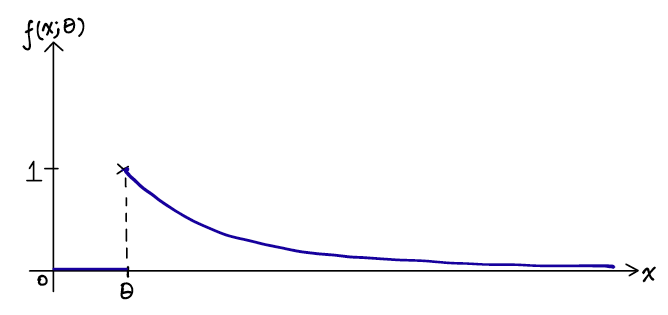
\includegraphics[scale=0.5]{3a.png}
	\item 
		For $x\ge \theta$ the cumulative distribution function $F(x;\theta) $ of $X_{1}$ is
		\begin{align*}
		F(x;\theta) &= \int^x_{-\infty} f(t;\theta) dt \\
		&=\int^x_{\theta} e^{(\theta-t)} dt \\
		&= -e^{\theta-t}\bigg |^x_\theta \\
		&=1-e^{\theta-x}
		\end{align*}
		Then
		\begin{align*}
		F_{X_{(1)}}(y;\theta) &= P(X_{(1)}\le y)\\
		&= 1 - P(X_{(1)}\ge y)\\
		&= 1 - P(X_1 \ge y, ... , X_n \ge y)\\
		&= 1 - \bigg[P(X_1 \ge y) \bigg]^n &  (i.i.d.)\\
		&= 1 - \bigg[ 1 - (1-e^{\theta-x}) \bigg]^n\\
		&= 1 - e^{n(\theta-x)}\\
		&= 1- e^{n\theta}e^{-nx}\\
		\end{align*}
		Therefore
		\begin{align*}
		f_{X_{(1)}}(x;\theta) &= \frac{d}{dx}F_{X_{(1)}}(y;\theta) \\
		&= -e^{n\theta}(-n)e^(-nx)\\
		&= ne^{n(\theta-x)}
		\end{align*}
		Hence
		\[
		f(z) = \left\{ 
			\begin{array}{rcl}
			ne^{n(\theta-x)} & \mbox{for}
			& x \ge \theta \\ 0 & \mbox{for} & x<\theta \\
			\end{array}\right.
		\]
	\item
		Since $X_1, ... , X_n$ are i.i.d. random variable with $f(x;\theta) = e^{\theta-x}I_{(-\infty,x]}(\theta) =  \left\{ 
			\begin{array}{rcl}
			ne^{n(\theta-x)} & \mbox{for}
			& x \ge \theta \\ 0 & \mbox{for} & x<\theta \\
			\end{array}\right.$
			\\Then the likelihood function is
			\begin{align*}
			L(x;\theta) &= \prod^n_{i=1} f( X_i;\theta) & (i.i.d)\\
			&=  \prod^n_{i=1} e^{\theta-x_i}I_{(-\infty,x_{(1)}]}(\theta) \\
			&= exp\bigg\{ n\theta - \sum^n_{i=1} x_t\bigg\}I_{(-\infty,x_{1}]}(\theta) 
			\end{align*}
		Let $\psi (\theta)$ be the ratio of the likelihood between two sample points {\bf x} , {\bf y}
		\begin{align*}
		\psi(\theta) = \frac{L(x;\theta)}{L(y;\theta)}= \frac{exp\{n\theta-\sum^n_{i=1}x_i\}I_{(-\infty,x_{1}]}(\theta) }{exp\{n\theta-\sum^n_{i=1}y_i\}I_{(-\infty,y_{1}]}(\theta)}=exp \bigg \{ \sum^n_{i=1}y_i-\sum^n_{i=1}x_i \bigg \} \frac{I_{(-\infty,x_{1}]}(\theta) }{I_{(-\infty,y_{1}]}(\theta)}
		\end{align*}
		For $x_{(1)}<y_{(1)}$,
		\[
		\psi (\theta) =
		\left\{ 
			\begin{array}{rcl}
			exp \bigg [ \sum^n_{i=1}y_i-\sum^n_{i=1}x_i \bigg ] & \mbox{for}
			& \theta \le x_{(1)} \\ 0 & \mbox{for} & x_{(1)}<\theta \le y_{(1)} \\
			\mbox{undefined} & \mbox{for}  & \theta> y_{(1)}  
			\end{array}\right.
		\]
		For $y_{(1)}<x_{(1)}$,
		\[
		\psi (\theta) =
		\left\{ 
			\begin{array}{rcl}
			exp \bigg [ \sum^n_{i=1}y_i-\sum^n_{i=1}x_i \bigg ] & \mbox{for}
			& \theta \le y_{(1)} \\ 0 & \mbox{for} & y_{(1)}<\theta \le x_{(1)} \\
			\mbox{undefined} & \mbox{for}  & \theta> x_{(1)}  
			\end{array}\right.
		\]
		If $x_{(1)} \not= y_{(1)}, \psi(\theta)$ is not a constant with respect to $\theta$.
		\\If $x_{(1)} = y_{(1)}$,
		\[
		\psi (\theta) = 
		\left\{ 
			\begin{array}{rcl}
			exp \bigg [ \sum^n_{i=1}y_i-\sum^n_{i=1}x_i \bigg ] & \mbox{for}
			& \theta \le x_{(1)} = y_{(1)} \\
			\mbox{undefined} & \mbox{for}  & \theta> x_{(1)}  = y_{(1)}
			\end{array}\right.
		\]
		$\psi (\theta)$ is constant with respect to $\theta$. Hence, by Lehmann-Schette's method, $X_{(1)}$ is a minimal sufficient statistic for $\theta$.
	\item
		\begin{align*}
		E_{\theta}[X_{(1)}] &= \int^\infty_\theta xf_{X_{(1)}}(x;\theta) dx \\
		&= \int^\infty_\theta x ne^{n(\theta-x)} dx \\
		&= ne^{n\theta}\int^\infty_\theta  x e^{-nx} dx\\
		&= e^{n\theta}\bigg( -xe^{-nx} \bigg|^\infty_\theta + \int^\infty_\theta e^{-nx}dx  \bigg) & \mbox{(by parts)}\\
		&= e^{n\theta}\bigg( \theta e^{-n\theta} + \frac{1}{n} e^{-n\theta}  \bigg)\\
		&= e^{n\theta}e^{-n\theta}\bigg( \theta +\frac{1}{n} \bigg)\\
		&= \theta +\frac{1}{n} 
		\end{align*}
	\item
		Let $g$ be a function from $[\theta,\infty)$ to $\mathbb{R}$ and suppose that $ E_{\theta}[g(X_{(1)}] = 0$ for all $\theta \in \mathbb{R}$, which means:
		\begin{align*}
		0&=\int^\infty_\theta g(t)f_{X_{(1)}}(t;\theta)dt\\
		&=\int^\infty_\theta g(t)ne^{n(\theta-t)}dt\\
		&=ne^{n\theta}\int^\infty_\theta g(t)e^{-nt}dt\\
		0&=\int^\infty_\theta g(t)e^{-nt}dt\\
		\end{align*}
		Differentiate both sides and apply the fundamental theorem of calculus,
		\begin{align*}
		0&=-g(\theta)e^{-n\theta} \\
		\end{align*}
		Therefore $g(\theta) = 0 $ for all $\theta \in \mathbb{R}$ since $e^{-\theta} >0$  for all $\theta \in \mathbb{R}$.
		\\Then   $g(x) = 0 $ for $x\in [\theta,\infty)$, so $Pr_{\theta}(g(X_{(1)}=0)=1$ for all $\theta \in \mathbb{R}$ and hence $X_{(1)}$ is complete.
		\\ From part (c), we have justified that $X_{(1)}$ is also minimal sufficient for $\theta$.
		\\Therefore, considering part (d) where $E_{\theta}[X_{(1)}] = \theta +\frac{1}{n}$ which means that in order to obtain UMVUE of $\theta$, we will need $W = X_{(1)}-\frac{1}{n}$ which will give us $E(W) = E(X_{(1)}-\frac{1}{n}) = E(X_{(1)})-\frac{1}{n} = \theta +\frac{1}{n}-\frac{1}{n} = \theta$ for all $\theta$.
		\\Then by the Lehmann-Scheffe Theorem, the UMVUE of $\theta$ is 
		\[E[W|X_{(1)}]= E[X_{(1)}-\frac{1}{n} |X_{(1)}] = E[X_{(1)}|X_{(1)}]-\frac{1}{n} = X_{(1)}-\frac{1}{n} 
		\]
\end{enumerate}
\section{Question 4}
\begin{enumerate}[(a)]
	\item Given that {\bf X} = $(X_1, X_2, ... , X_n)$ is a sample of $n$ i.i.d observations from Bernoulli distribution with probability of success $\theta$.
	\\Suppose that an unbiased estimator of $\tau(\theta) = \frac{\theta}{1-\theta}$ did exist, then by Rao- Blackwell Theorem, an unbiased estimator {\bf T} of $\tau(\theta)= \frac{\theta}{1-\theta}$ will exist, where {\bf T} is a function of sufficient statistic.
	\\Considering the statistic $\tilde{X} = \sum^n_{i=1}X_i \sim Bin(n,\theta)$ since each $X$ is a $Bern(\theta)$.
	\\Then
	\begin{align*}
	E_\theta[{\bf T}(\tilde{X})] &= \tau(\theta) & \mbox{(using  Rao- Blackwell Theorem)}\\
	\sum^n_{x=0}T(x)\dbinom{n}{x} \theta^x(1-\theta)^{n-x}&=\frac{\theta}{1-\theta}  & \forall \theta \in (0,\infty)
	\end{align*}
	However, this is impossible, since as $\theta \rightarrow 1$ the L.H.S of the above equation will be equal to {\bf T$(1)$} which is a finite constant (M)
	\[
	\lim_{\theta \rightarrow 1} \sum^n_{x=0}T(x)\dbinom{n}{x} \theta^x(1-\theta)^{n-x} = T(1) = M
	\]
	While the R.H.S (odd ratio) can be larger than any finite constant M (given from the hints in the question).
	\\This is a contradiction as L.H.S $\not=$ R.H.S hence no unbiased estimator of $\tau(\theta)=\frac{\theta}{1-\theta}$ exists.
	\item
		First obtain the MLE of $\theta$:
		\begin{align*}
		0 &= V({\bf X}, \hat{\theta}) \\
		&= \frac{\sum^n_{i=1} X_i}{\hat{\theta}} - \frac{n-\sum^n_{i=1}X_i}{1-\hat{\theta}}\\
		\frac{\sum^n_{i=1} X_i}{\hat{\theta}} &= \frac{n-\sum^n_{i=1} X_i}{1-\hat{\theta}}\\
		\sum^n_{i=1} X_i - \hat{\theta} \sum^n_{i=1} X_i &= n\hat{\theta} - \hat{\theta} \sum^n_{i=1} X_i\\
		\hat{\theta} &= \frac{\sum^n_{i=1} X_i}{n}\\
		\hat{\theta} &= \bar{X} \\
		\end{align*}
		Then using the transformation invariance property of the MLE, we can obtain the MLE $\hat{\tau}$ of $\tau(\theta)$ which is,
		\[
		\hat{\tau}_{\bf MLE} = \tau(\hat{\theta})= \frac{\hat{\theta}}{1-\hat{\theta}} = \frac{\bar{X}}{1-\bar{X}}
		\]
		Now as MLE is asymptotically normal, unbiased and efficient, so by delta method, the asymptotic distribution is
		\[
		\sqrt{n}(\hat{\tau} - \tau(\theta)) \xrightarrow{d} N\bigg( 0 , \bigg[ \frac{\partial \tau(\theta)}{\partial \theta} \bigg]^2 I_{X_1}^{-1}(\theta)\bigg)
		\]
		where 
		\[
		\frac{\partial \tau(\theta)}{\partial \theta} = \frac{\partial}{\partial \theta} \bigg(  \frac{\theta}{1-\theta} \bigg) = \frac{1-\theta - (-1)\theta}{(1-\theta)^2} = \frac{1}{(1-\theta)^2}
		\]
		and
		\begin{align*}
		I_{X}(\theta) &= E\bigg[-\frac{\partial}{\partial \theta} V(\bf{X},\theta) \bigg] = E\bigg[-\frac{\partial}{\partial \theta} \bigg( \frac{\sum^n_{i=1} X_i}{\hat{\theta}} - \frac{n-\sum^n_{i=1}X_i}{1-\hat{\theta}} \bigg) \bigg]\\ &= E\bigg[ \frac{\sum^n_{i=1} X_i}{\hat{\theta}^2}+\frac{n-\sum^n_{i=1} X_i}{(1-\theta)^2} \bigg] = \frac{n\theta }{\theta^2}+\frac{n-n\theta}{(1-\theta)^2} &  (\mbox{we know that } n\hat{\theta} = \sum^n_{i=1}X_i)\\
		&= n\bigg(\frac{1}{\theta} + \frac{1}{1-\theta}  \bigg) = \frac{n}{\theta(1-\theta)} 
		\end{align*}
		therefore
		\[
		I_{X_1}(\theta) = \frac{1}{\theta(1-\theta)} 
		\]
		Substitute all the calculation back we obtain the distribution as follow:
		\[
		\sqrt{n}(\hat{\tau} - \tau(\theta)) \xrightarrow{d} N\bigg( 0 , \bigg[ \frac{1}{(1-\theta)^2}\bigg]^2 \theta(1-\theta) \bigg)= N\bigg(0, \frac{\theta}{(1-\theta)^3} \bigg) 
		\]
		Therefore, the asymptotic 90\% confidence interval for $\tau(\theta)$ is 
		\[
		(\hat{\tau} \pm \Phi^{-1}(0.95)\hat{se}(\hat{\tau})) =\bigg(\frac{\theta}{1-\theta} \pm \Phi^{-1}(0.95) \sqrt{\frac{\theta}{(1-\theta)^3} } \bigg)
		\]
\end{enumerate}
\section{Question 5}
\begin{enumerate}[(a)]
	\item
	\begin{enumerate}[(i)]
		\item
			Since it is given that the common density function is $f(x;\theta) = \theta x^{(\theta-1)}$ for  $0<x<1$ and $\theta>0$, then  it can be easily be represented in the form of exponential family
			\begin{align*}
				f(x;\theta) &= \theta x^{(\theta-1)} \\
				&= exp[ log( \theta x^{(\theta-1)} )] \\
				&= exp[ log(\theta)+(\theta-1)log(x)]\\
				&= \theta \times e^{(\theta-1)log(x)}\\
				&= a(\theta)b(x) exp[c(\theta)d(X)]\\
			\end{align*}
			It is clear that $a(\theta) = \theta$, $b(x)=1$, $c(\theta)=\theta-1$, $d(X)=log(x)$. Therefore, the distribution belongs to the exponential family. So the statistic will be $T = \sum^n_{i=1}d(X_i) =  \sum^n_{i=1} log(X_i)$ and it is complete and minimal sufficient. To double check for minimal sufficient we can look at the likelihood function:
			\begin{align*}
			L({\bf x}, \theta) &= \prod^n_{i=1}f(x_i;\theta) & \mbox{as }X_1, ... , X_n\mbox{ are i.i.d.)}\\
			&= \prod^n_{i=1} \theta e^{(\theta-1)log(x_i)}\\
			&=\theta^n exp\bigg\{(\theta-1)\sum^n_{i=1} log x_i \bigg\}
			\end{align*}
			Then the ratio of the likelihoods for data vectors {\bf x} and {\bf y} is
			\begin{align*}
			 \frac{L({\bf x};\theta)}{L({\bf y};\theta)}&=\frac{\theta^n exp\bigg\{(\theta-1)\sum^n_{i=1} log x_i \bigg\}}{\theta^n exp\bigg\{(\theta-1)\sum^n_{i=1} log y_i \bigg\}}\\
			&=exp\bigg\{\sum^n_{i=1} log x_i-\sum^n_{i=1} log y_i \bigg\}\\
			\end{align*}
			as it is independent of $\theta$ if and only if $\sum^n_{i=1} log x_i=\sum^n_{i=1} log y_i$. Hence , by the Lehmann and Scheffe theorem, $T = \sum^n_{i=1}d(X_i) =  \sum^n_{i=1} log(X_i)$ is a minimal sufficient statistic for $\theta$.
		\item
			Suppose $W= -log X_1$ is a an unbiased estimator of $\tau(\theta) = \frac{1}{\theta}$, which means we must have $E[W] = \frac{1}{\theta}$. Now check the condition:
			\begin{align*}
			E[W] &= E[ -log X_1]\\
			&= \int^1_0 (-logx) \theta x^{(\theta-1)} dx\\
			&= \int^\infty_0 w \theta e^{-w\theta} dw & \mbox{by substitution, $w= -log x$} \\
			&= we^{-w\theta}\bigg|^\infty_0+\int^\infty_0 e^{-w\theta} dw & \mbox{by parts, } u=w, v'=e^{-w\theta}\\
			&=\frac{e^-w\theta}{\theta} \bigg|^\infty_0\\
			&= \frac{1}{\theta}\\
			\end{align*}
			Therefore, $W = -log X_1$ is an unbiased estimator of $\frac{1}{\theta}$.
			\\Now, we first look at Variance of $\sqrt{W}$
			\begin{align*}
				Var[\sqrt{W}]&>0 & \mbox{(since variance is positive and is only equal to zero if its not random)}\\
				E[\sqrt{W}^2] - E[\sqrt{W}]^2&>0\\
				E[\sqrt{W}^2]&>E[\sqrt{W}]^2\\
				\frac{1}{\sqrt{\theta}}&>E[\sqrt{W}]
			\end{align*}			 
			This means that $\sqrt{W}$ is a biased estimator of $\xi(\theta)=\frac{1}{\sqrt{\theta}}$ since $E[\sqrt{W}]<\frac{1}{\sqrt{\theta}}$.
		\item
			Suppose $X_1 \sim U[0,1]$ and $W = -log(X_1)$, then consider the cumulative distribution function of W will be as follow
			\begin{align*}
			F_W(w) &= Pr(W<w)\\
			&= Pr(-logX<w) & \mbox{(substitute $W = -logX$)}\\
			&= 1- Pr(X<e^{-w})\\
			&=1-F_X[e^{-w}]\\
			\frac{\partial}{\partial W} F_W(w)&=\frac{\partial}{\partial W}\bigg[1-F_X[e^{-w}] \bigg] 
			\end{align*}
			To obtain $F_X[e^{-w}]$ we can do the follow:
			\begin{align*}
			F_X(x) & = \int^x_0 \theta t^{(\theta-1)}dt\\
			&= \theta \int^x_0 t^{(\theta-1)}dt\\
			&= x^\theta
			\end{align*}
			Then applied that into the previous equation for cdf of W:
			\begin{align*}
			f_W(w)&=\frac{\partial}{\partial W}\bigg[1-[e^{-w\theta}] \bigg] \\
			&= \theta e^{-w\theta}
			\end{align*}			
			which is the probability density of a Exponential distribution with parameter $\theta$.
		\item
			From previous part we found that $T$ is a complete sufficient statistic for $\theta$ and $W$ is an unbiased estimator of $\tau(\theta)$. 
			Note that since $W\sim exp(rate = \theta)$ and therefore,
			\[
			T= \sum^n_{i=1} -log(X_i) \sim \Gamma(n,\theta).
			\]
			Then By Lehmann-Scheffe theorem, if we can find a function of T whose expected value is $\frac{1}{\theta}$, we have an UMVUE for $\tau(\theta)=\frac{1}{\theta}$.
			First look at $E(T)$:
			\[
			E[T] = E\bigg[ \sum^n_{i=1} -log(X_i) \bigg] =  \sum^n_{i=1} E\bigg[-log(X_i) \bigg] \stackrel{iid}{=} nE[-log(X_1)]=nE[W]
			\]
			since we know that $W = -log X_1$ is an unbiased estimator of $\frac{1}{\theta}$, that means
			\[
			E[T] = nE[W] = \frac{n}{\theta}
			\]
			Therefore, using the Lehmann-Scheffe Theorem, we have $\frac{T}{n}=\frac{-\sum^n_{i=1} logX_i}{n}$ as the UMVUE for $\frac{1}{\theta}$. It can be checked by looking at the expected value of $\frac{T}{n}$ as follow:
			\[
			E\bigg[\frac{T}{n}\bigg] =\frac{E[T]}{n}=\frac{n/\theta}{n}=\frac{1}{\theta}
			\]
		\item
			For the UMVUE of $\bar{\tau} = \theta$, we first consider $E[ \frac{1}{T}]$
			\\Note that $W = -logX_1 \sim \Gamma(1,\theta)$ and $T = -\sum^n_{i=1} logX_i \sim \Gamma(n,\theta)$ since they are i.i.d distributed.
			\begin{align*}
			E\bigg[ \frac{1}{T} \bigg] &= \int^\infty_0  \frac{1}{t}  f_T(t) dt \\
			&= \int^\infty_0 \frac{1}{t}  \frac{1}{\Gamma(n)}\theta^nt^{n-1}e^{-\theta t} dt\\
			&= \frac{\Gamma(n-1)}{\Gamma(n)} \theta \int^\infty_0 \frac{1}{\Gamma(n-1)}\theta^{n-1}t^{n-2}e^{-\theta t} dt\\
			&= \frac{\Gamma(n-1)}{\Gamma(n)} \theta \times 1 & \mbox{\bigg(pdf of $\Gamma(n-1,\theta)\bigg)$}\\
			&=\frac{(n-2)!}{(n-1)!}\theta\\
			&= \frac{\theta}{n-1}
			\end{align*}
			Therefore, 
			\[
			(n-1)\frac{1}{T} = \frac{n-1}{\sum^n_{i=1} -logX_i}
			\]
			is a function of the complete and sufficient statistic $T$ that is unbiased for $\theta$. So, by the Lehmann-Scheffe Theorem, we have 
			\[
			\hat{\theta}_{UMVUE} = \frac{n-1}{\sum^n_{i=1} -logX_i}
			\]
	\end{enumerate}
	\item
		Since it is given that n i.i.d. samples are taken from $N(\mu,\theta^2)$ with known $\mu$. Then the probability density function for $X_i$ is 
		\begin{align*}
		f(x;\theta) &= \frac{1}{\theta\sqrt{2\pi}}exp\bigg\{-\frac{(x-\mu)^2}{2\theta^2} \bigg\} & \mbox{for }  x \in \mathbb{R} \mbox{ and }\theta>0
		\end{align*}
		Then  it can be easily be represented in the form of exponential family
			\begin{align*}
				f(x;\theta) &=\frac{1}{\theta\sqrt{2\pi}}exp\bigg\{-\frac{(x-\mu)^2}{2\theta^2} \bigg\}  \\
				&= a(\theta)b(x) exp[c(\theta)d(X)]
			\end{align*}
			It is clear that $a(\theta) = \frac{1}{\theta}$, $b(x)=1\frac{1}{\sqrt{2\pi}}$, $c(\theta)=-\frac{1}{2\theta^2}$, $d(X)=(x-\mu^2)$. Therefore, the distribution belongs to the exponential family. So the statistic will be $T = \sum^n_{i=1}d(X_i) =\sum^n_{i=1} (X_i-\mu)^2$ and it is a complete and minimal sufficient statistic.
			\newpage Now consider $S^2$
			\[
			S^2 = \frac{1}{n}\sum^n_{i=1} (X_i-\mu)^2 = \frac{T}{n}
			\]
			as it is a function of T, it is also a complete and minimal sufficient statistic.
			\\Now we want to find the distribution of $S^2$, but first note that $X_i \sim N(\mu,\theta^2)$ where $i = 1,...., n$.
			Then we can standardised the distribution of $X_i$ which is
			\begin{align*}
			X_i& \sim N(\mu,\theta^2)\\
			\frac{X_i-\mu}{\theta} &\sim  N(0,1)
			\end{align*}
			Then we can square it to form something similar to $S^2$
			\[
			\frac{(X_i-\mu)^2}{\theta^2} \sim \chi^2_{(1)}
			\]
			Since square of a Normal random variable will give a 1 degree Chi-Square random variable. Then we are able to deduce that the sum of n Chi-Square random variable will be a n degree Chi-Square random variable which is
			\[
			\frac{\sum^n_{i=1}(X_i-\mu)^2}{\theta^2} \sim \chi^2_{(n)}
			\]
			Therefore,
			\[
			S^2 =  \frac{1}{n}\sum^n_{i=1} (X_i-\mu)^2  \sim  \frac{\theta^2}{n}\chi^2_{(n)}
			\]
			Hence
			\[
			\frac{n}{\theta^2}S^2 \sim \chi^2_n.
			\]
			Now by the Lehmann-Scheffe theorem, if we can find a function of $S$ whose expected value is $\theta$, then we have an UMVUE for $\theta$.
			\\It is not clear which function to choose. So we can first find $E[\frac{n}{\theta^2}S^2]$. Then try to multiply or divide to make a function of S that is unbiased for $\theta$.
			\\Note that in order to find $E[\frac{n}{\theta^2}S^2]$, it is essential to obtain the moment generating function of Chi-Square distribution with n degrees of freedom first.
			Let the m.g.f of Chi-Square distribution be $m_Y(t)$
			\begin{align*}
			m_{Y}(t) &= E[e^{tY}]\\
			&= \int^\infty_{-\infty} e^{tY} f_Y (y) dy\\
			&= \frac{1}{2^{n/2}\Gamma(\frac{n}{2})} \int^\infty_0 e^{tY} y^{\frac{n}{2}-1} e^{-\frac{1}{2}y} dy\\
			&= \frac{1}{2^{n/2}\Gamma(\frac{n}{2})} \int^\infty_0  y^{\frac{n}{2}-1} exp\bigg\{{-\bigg(\frac{1}{2}-t\bigg)y}\bigg\} dy\\
			&= \frac{1}{2^{n/2}\Gamma(\frac{n}{2})} \int^\infty_0  \bigg(\frac{2}{1-2t}u \bigg)^{\frac{n}{2}-1} e^{-u}\frac{2}{1-2t}du & \bigg( \mbox{changing variable : }u= (\frac{1}{2}-t)y\bigg)\\
			&= \frac{1}{2^{n/2}\Gamma(\frac{n}{2})} \int^\infty_0  \bigg(\frac{2}{1-2t} \bigg)^{\frac{n}{2}}u^{^{\frac{n}{2}-1}} e^{-u} du \\
			&=\frac{1}{2^{n/2}\Gamma(\frac{n}{2})} \bigg(\frac{2}{1-2t} \bigg)^{\frac{n}{2}} \int^\infty_0  u^{^{\frac{n}{2}-1}} e^{-u} du \\
			&=\frac{1}{2^{n/2}\Gamma(\frac{n}{2})} \bigg(\frac{2}{1-2t} \bigg)^{\frac{n}{2}} \Gamma\bigg(\frac{n}{2}\bigg)  & \bigg(\mbox{ by definition of Gamma function}\bigg)\\
			&=(1-2t)^{-\frac{n}{2}}
			\end{align*}
			Hence we can now find the $m^{th}$ non-central moment using the m.g.f $ (1-2t)^{-\frac{n}{2}}$ of Chi-Square distribution with n degree of freedoms
			\begin{align*}
			E[(\frac{n}{\theta^2}S^2)^m]&=   n(n+2)(n+4)...(n+2m-2) = 2^m \frac{\Gamma(m+\frac{n}{2})}{\Gamma(\frac{n}{2})}
			\end{align*}
			Apply the above formula, we can obtain 
			\begin{align*}
			E[\frac{n}{\theta^2}S^2]&=  2 \frac{\Gamma(1+\frac{n}{2})}{\Gamma(\frac{n}{2})}\\
			E[S^2] & =  2 \frac{\Gamma(1+\frac{n}{2})}{\Gamma(\frac{n}{2})} \frac{\theta^2}{n}
			\end{align*}
			However, we are looking for UMVUE for $\theta$ therefore we should find $E[S]$ instead:
			\begin{align*}
			E\bigg[\bigg(\frac{n}{\theta^2}S^2\bigg)^{1/2}\bigg]&=  2^{\frac{1}{2}} \frac{\Gamma(\frac{1}{2}+\frac{n}{2})}{\Gamma(\frac{n}{2})}\\
			E[S] & =  \sqrt{\frac{2}{n}} \frac{\Gamma(\frac{n+1}{2})}{\Gamma(\frac{n}{2})} \theta
			\end{align*}
			Therefore,
			\[
			 \sqrt{\frac{n}{2}} \frac{\Gamma(\frac{n}{2})}{\Gamma(\frac{n+1}{2})}S = \sqrt{\frac{n}{2}} \frac{\Gamma(\frac{n}{2})}{\Gamma(\frac{n+1}{2})} \sqrt{\frac{T}{n}}=  \sqrt{\frac{n}{2}} \frac{\Gamma(\frac{n}{2})}{\Gamma(\frac{n+1}{2})} \sqrt{\frac{1}{n}\sum^n_{i=1} (X_i-\mu)^2}
			\]
			is a function of the complete and sufficient statistic S that is unbiased for $\theta$. So by the Lehmann-Scheffe Theorem, we have
			\[
			\hat{\theta}_{UMVUE} = \sqrt{\frac{n}{2}} \frac{\Gamma(\frac{n}{2})}{\Gamma(\frac{n+1}{2})}S
			\]
			where $S^2 = \frac{1}{n}\sum^n_{i=1} (X_i-\mu)^2$ as given in the question.
		\newpage
		\item
			From the previous part, we have $S^2 = \frac{1}{n}\sum^n_{i=1} (X_i-\mu)^2$, however, since $\mu$ is unknown. We have to consider the sample variance and sample mean instead of the population variance and population mean. To check if the sample variance is unbiased:
			\begin{align*}
			s^2 &=  \frac{1}{n-1}\sum^n_{i=1} (X_i-\bar{X})^2 \\
			E[s^2] & =  \frac{1}{n-1}\sum^n_{i=1} E[(X_i-\bar{X})^2] \\
			& =  \frac{1}{n-1}\sum^n_{i=1} E[X_i^2-2X_i\bar{X}+\bar{X}^2] \\
			&= \frac{1}{n-1}\sum^n_{i=1} E[X_i^2]-2E[X_i\bar{X}]+E[\bar{X^2}] \\
			&\bigg( \mbox{using the identity:}E[X_i^2]=Var[X_i]+E[X_i]^2\bigg)\\
			&= \frac{1}{n-1}\sum^n_{i=1} Var[X_i]+E[X_i]^2 - 2E[X_i\frac{1}{n}\sum^n_{j=1}X_j]+E[\bar{X^2}] \\
			&=  \frac{1}{n-1}\sum^n_{i=1} Var[X_i]+E[X_i]^2 - \frac{2}{n}\sum^n_{j=1}E[X_iX_j]+E[\bar{X^2}]
			\end{align*}
		\[
		 \bigg( E[X_iX_j] = Cov(X_i,X_j)+E[X_i]E[X_j] = 
		\left\{
			\begin{array}{rcl}
			\theta^2 + \mu^2 & \mbox{for}
			& i=j \\
			\mu^2 & \mbox{for}  & i  \not= j
			\end{array}\right.  \bigg)
		\]
		\begin{align*}
		E[s^2] &=  \frac{1}{n-1}\sum^n_{i=1} Var[X_i]+E[X_i]^2 - \frac{2}{n}\sum^n_{j=1}E[X_iX_j]+Var[\bar{X}]+E[\bar{X}]^2 \\
		&=\frac{1}{n-1}\sum^n_{i=1}\bigg( \theta^2+\mu^2 - \frac{2}{n}\theta^2+2\mu^2+\frac{\theta^2}{n} +\mu^2\bigg)\\
		&=\frac{1}{n-1}\sum^n_{i=1}\bigg( \theta^2 - \frac{\theta^2}{n}\bigg)\\
		&=\frac{1}{n-1}\sum^n_{i=1}\bigg( \theta^2 \bigg( 1- \frac{1}{n}\bigg)\bigg)\\
		&=\frac{1}{n-1}\sum^n_{i=1}\bigg( \theta^2 \bigg( 1- \frac{1}{n}\bigg)\bigg)\\
		&=\frac{ \theta^2}{n-1}\sum^n_{i=1}\bigg( \frac{n-1}{n}\bigg)\\
		&=\frac{ \theta^2n}{n-1}\bigg( \frac{n-1}{n}\bigg)\\
		&=\theta^2
		\end{align*}
		Now obtain the distribution of $s^2$
			\begin{align*}
			X_i& \sim N(\mu,\theta^2)\\
			\frac{X_i-\bar{X}}{\theta} &\sim  N(0,1)
			\end{align*}
			Then we can square it to form something similar to $s^2$
			\[
			\frac{(X_i-\mu)^2}{\theta^2} \sim \chi^2_{(1)}
			\]
			Since square of a Normal random variable will give a 1 degree Chi-Square random variable. Then we are able to deduce that the sum of n Chi-Square random variable will be a n degree Chi-Square random variable which is
			\[
			\frac{\sum^n_{i=1}(X_i-\mu)^2}{\theta^2} \sim \chi^2_{(n)}
			\]
			Therefore,
			\[
			s^2 =  \frac{1}{n-1}\sum^n_{i=1} (X_i-\mu)^2  \sim  \frac{\theta^2}{n-1}\chi^2_{(n)}
			\]
			Hence
			\[
			\frac{n}{\theta^2}S^2 \sim \chi^2_n.
			\]
			Now by the Lehmann-Scheffe theorem, if we can find a function of $S$ whose expected value is $\theta$, then we have an UMVUE for $\theta$.
\end{enumerate}
\end{document}
